\documentclass[a4paper,10pt]{scrartcl}[2003/01/01]
\usepackage[ngerman]{babel}
\usepackage[T1]{fontenc}
\usepackage{inputenc}
\usepackage{graphicx}
\usepackage{listings}
\usepackage{enumerate}
\usepackage{pstricks}
\title{Software Architectures}
\subtitle{Exercise 6}
\author{ Felix Baumann \\ Manuel Gottschlich \\  Alexey Gy\"ori 352678 \\ Vincent Wehrwein \\ Markus Weller 352466}
\begin{document}
    \maketitle
    
    \section*{Aufgabe 6.1}
        \subsection*{a)}
        \subsection*{b)}
    \section*{Aufgabe 6.2}
        \subsection*{a)}
        \subsection*{b)}
        \newpage
    \section*{Aufgabe 6.3}
        \subsection*{a)}
        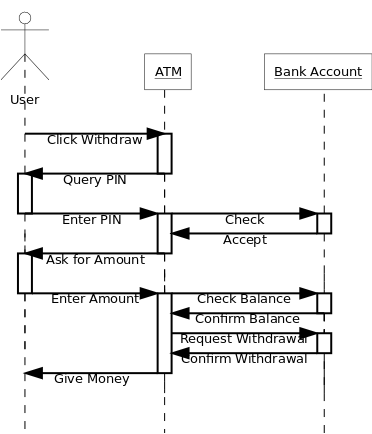
\includegraphics[scale=0.5]{Diagram1}
        \subsection*{b)}
        Sequence Diagrams are for showing complex interactions between entities.\\
        State Diagrams are for showing complex choices with the respective outcomes.\\
        
        It is hard to show different scenarios within one sequence diagram.
        \subsection*{c)}
        Class Diagrams usually only show the interfaces and variables of a class and have no information about the implementation of the functions.\\
        State and sequence are for explaining the implementation of the functions to the interfaces.
\end{document}